\begin{figure}
	
	\floatbox{figure}[\FBwidth]
	{
		\caption{Readability of authors' $t$th publication (draft and final versions)}\label{figure6}
	}
	{
		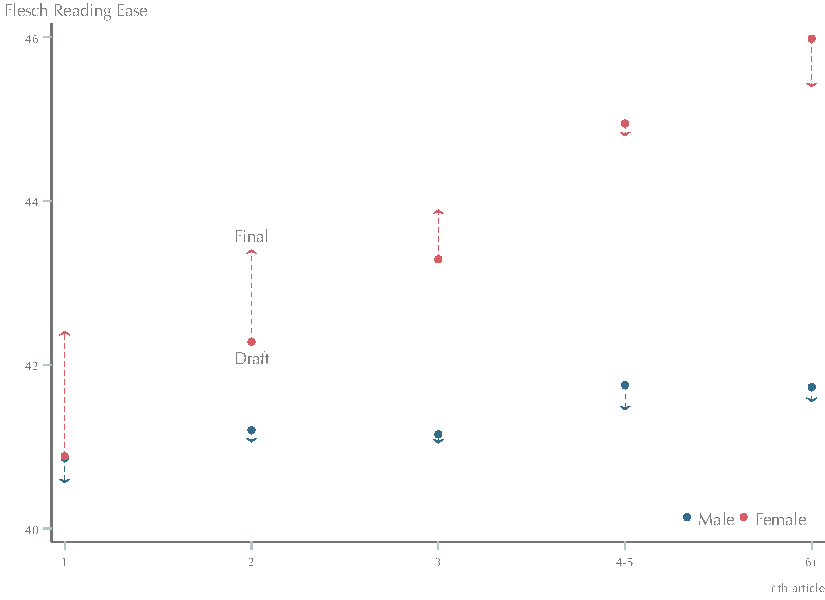
\includegraphics[width=12.3cm]{$HOME/Dropbox/Readability/draft/pdf/figure6.pdf}
		\floatfoot{\tiny \textit{Notes}. Sample 4,289 observations; 1,988 and 1,986 distinct NBER working papers and published articles, respectively; 1,840 distinct authors. Flesch Reading Ease marginal mean scores for authors' first, second, third, 4th--5th and sixth and up publications in the data. Solid circles denote estimated readability of NBER working papers from FGLS estimation of~\autoref{equation14}; arrow tips show the estimated readability in published versions of the same papers. Controls are: editor, year, journal, journal and year interactions, English fluency dummies and quality controls (citation count and $\text{max. }T_j$). Regression weighted by $1/N_j$. Pink represents women co-authoring only with other women; blue are men co-authoring only with other men.}
	}
\end{figure}